\chapter{Ventanas de la aplicación}

En este capítulo se explicarán las ventanas de las que dispone el programa.

\section{Ventana Principal}

La ventana principal aparece al inicio del programa y es utilizada como interfaz básica de interactuación con el usuario. En ella se incluyen botones para acceder al resto de ventanas que en este capítulo se presentan.\\

\begin{figure}[!h]
\begin{center}
\includegraphics*[height=1.4cm]{images/mprincipal.png}
\caption{Ventana principal inicial de la aplicación \emph{surcos}}\label{mainWindow}
\end{center}
\end{figure}

\begin{table}[h]\footnotesize
\begin{center}
\begin{tabular}{llr}
\hline
\multicolumn{2}{c}{Elemento} \\
\cline{1-2}
Icono & Acción & Funcionalidad \\
\hline
Salir & Click & Salir de la aplicación\\
Abrir & Click & Abrir ventana de carga de caso \\
Configurar & Click & Abrir ventana de configuración de caso \\
Ejecutar & Click & Ejecutar caso \\
Gráficos & Click & Abrir ventana de visualización de resultados  \\
Sumario & Click & Abrir ventana de sumario \\
Ayuda & Click & Créditos \\
\hline
\end{tabular}
\end{center}
  \caption{Descripción de las diferentes acciones disponibles en el menú principal de la aplicación \emph{surcos}}\label{mainWindowIcons}
\end{table}

A través de los iconos de la tabla \ref{mainWindowIcons} podemos acceder a las diferentes funcionalidades del programa.\\
\section{Configuración de caso}
\subsection{Ventana Configuración de Geometría}

El programa \emph{surcos} simula riego en redes de surcos en tablares de forma cuadrilátera. En la ventana de configuración de geometría (ver figura \ref{geomWindow}), podemos modificar la topografía del problema modificando los cuatro vértices que definen el tablar.

\begin{figure}[!h]
\begin{center}
\includegraphics*[width=\textwidth]{images/confGeom.png}
\qquad
\caption{Ventana de configuración de geometría}\label{geomWindow}
\end{center}
\end{figure}

Como puede verse en la figura \ref{geomWindow}, el surco de distribución se localiza entre los puntos 1 y 2 y el surco de recirculación, si lo hubiera, entre los puntos 3 y 4. Los surcos de riego se localizan perpendicularmente a los anteriores.

\subsection{Ventana Configuración de surcos}

\begin{figure}[!h]
\begin{center}
\includegraphics*[width=\textwidth]{images/confSurco.png}
\qquad
\caption{Ventana de configuración de surcos}\label{confSurcos}
\end{center}
\end{figure}

En la ventana \ref{confSurcos} tenemos las propiedades de los surcos que vamos a simular desglosados en tres tipos: Distribución, recirculación y riego (siendo éste último el que define los surcos de riego propiamente). Estas opciones estarán activadas o desactivadas en función de que existan o no tanto surcos de riego como  surco de recirculación.

Las propiedades configurables para los surcos son las que se recogen en la figura \ref{confSurcos}.

\subsection{Ventana Configuración de entradas}

\begin{figure}[!h]
\begin{center}
\includegraphics*[width=\textwidth]{images/confInput.png}
\qquad
\caption{Ventana de configuración de las entradas}\label{input}
\end{center}
\end{figure}

En la ventana \ref{input} se configuran las entradas de agua y fertilizante. Cada entrada está definida por un punto del tablar, los tiempos inicial y final de la descarga, y un caudal constante. Este caudal es  volumétrico en el caso del agua y másico en el caso del fertilizante.

Es posible tratar hidrogramas más complejos definiendo varias entradas asociadas al mismo punto geométrico con el objeto de que se forme un hidrograma final como la suma de cada uno de ellos. 


\subsection{Ventana Configuración de fertilizante}

\begin{figure}[!h]
\begin{center}
\includegraphics*[width=\textwidth]{images/confFerti.png}
\qquad
\caption{Ventana de configuración de fertilizante}\label{ferti}
\end{center}
\end{figure}

La ventana \ref{ferti} sirve para definir la solubilidad del fertilizante. 

\subsection{Ventana Configuración de sondas}

\begin{figure}[!h]
\begin{center}
\includegraphics*[width=\textwidth]{images/confSondas.png}
\qquad
\caption{Ventana de configuración de sondas}\label{sondas}
\end{center}
\end{figure}

En la ventana \ref{sondas} se pueden definir el número de sondas que vamos a utilizar, así como las posiciones geométricas de las mismas. Nótese que si el punto cae fuera del surco, se aproximará la posición a la más cercana dentro del tablar. 

\subsection{Ventana Configuración de parámetros avanzados}

\begin{figure}[!h]
\begin{center}
\includegraphics*[width=\textwidth]{images/confParam.png}
\qquad
\caption{Ventana de configuración de parámetros avanzados}\label{param}
\end{center}
\end{figure}

En la ventana \ref{param} se recogen las opciones de configuración de la simulación. En ella, podemos modificar los valores relacionados con la simulación numérica.

\begin{description}
\item{Tiempo máximo de duración de la simulación}: Normalmente el programa \emph{surcos} simula hasta que todo el agua se ha infiltrado en el terreno. Para evitar simulaciones demasiado largas, este parámetro permite definir el tiempo máximo en segundos en el que se aborta la simulación, aunque quede agua sin infiltrar en el sistema.
\item{CFL}: Parámetro numérico adimensional proporcional al paso de tiempo utilizado por el método matemático de resolución. Deben usarse valores entre 0 y 1. Valores cercanos a 1 son óptimos. Valores muy bajos pueden ralentizar considerablemente la ejecución.
\item{Periodo de volcado de datos}: Intervalo de tiempo de simulación cada cuanto se vuelcan los resultados numéricos en ficheros.
\item{Número de celdas del canal de distribución (entre surcos)}: Número de celdas que contiene la malla en los canales de distribución y de recirculación entre cada 2 confluencias con los surcos de riego.
\item{Número de celdas de los surcos de riego}: Número de celdas que contiene la malla en cada surco de riego.
\end{description}

De ellos, es importante tener en cuenta que aparece la condición CFL relacionada con la estabilidad numérica del método y la cual es necesario que sea menor que 1 $(CFL < 1)$. Además aparece un valor para seleccionar en el número de celdas para los distintos surcos. Es necesario tener en cuenta que este valor está relacionado con la calidad de la solución pero también con la duración del cálculo. Otro de los valores es la periodicidad de los volcados, de tal forma que podremos obtener $ n=\frac{t_s}{p_v}$ instantaneas de evolución, siendo $ t_s $ el tiempo de simulación y $ p_v $ el periodo de volcado. 

Los números de celdas también son decisivos en la velocidad de cálculo de la simulación. Un número excesivamente grande ralentiza considerablemente la simulación mientras que con un número pequeño se pierde precisión. 

\section{Simulación}

La simulación del caso, previa configuración, se realizará mediante el botón ejecutar del menú principal:

\includegraphics[height=0.4cm]{images/gtk-execute.png}

\section{Visualización de resultados}

%El programa puede mostrar tres tipos de resultados. El primero de ellos es modo textual y los otros dos son en modo gráfico

\subsection{Gráficas de resultados}

Las gráficas se controlan desde la ventana \ref{barraRepres}, donde se dispone de un dial para controlar el paso de tiempo representado en las variables que evolucionan con el tiempo. Además existe la posibilidad de seleccionar el surco, la variable o la sonda a representar. 

Se nos permite también guardar las gráficas pulsando en el botón que está al fondo del diálogo. En este case se guarda una imagen de la gráfica que hay en pantalla en un fichero en formato \emph{png}.

\begin{figure}[!h]
\begin{center}
\includegraphics*[width=\textwidth]{images/menuRepres.png}
\qquad
\caption{Ventana de selección de representación}\label{barraRepres}
\end{center}
\end{figure}

El programa \emph{Surcos} soporta tres tipos de representación. La primera de ellas es un mapa que representa de manera bidimensional la geometría de la red de surcos, posibilitando al usuario la representación de las variables descritas en la tabla \ref{tableVariablesMapa}.

\begin{table}[h]\footnotesize
\begin{center}
\begin{tabular}{ll}
\hline
Variable & Unidades \\
\hline
Calado & $m$ \\
Concentración de fertilizante & $ kg/m^3 $\\
Volumen de agua infiltrada por longitud de surco & $ m^2 $ \\
Masa de soluto por unidad de longitud & $ kg/m $ \\
\hline
\end{tabular}
\end{center}
  \caption{Variables visualizables en mapa de red de surcos}\label{tableVariablesMapa}
\end{table}

\begin{figure}[!h]
\begin{center}
\includegraphics*[width=\textwidth]{images/evo1.png}
\qquad
\caption{Ejemplo de representación en mapa de la variable calado}\label{evo1}
\end{center}
\end{figure}

Las otras dos son representaciones cartesianas de perfil longitudinal en los diferentes surcos y evoloución temporal en las diferentes sondas.

Las variables representables en el perfil longitudinal son las que aparecen en la tabla \ref{tableVariables2}.

\begin{table}[h]\footnotesize
\begin{center}
\begin{tabular}{ll}
\hline
Variable & Unidades\\
\hline
Calado & $m$ \\
Caudal & $ m^3/s $\\
Nivel (Cotas superficial y de fondo) & $ m $\\
Concentración de fertilizante & $ kg/m^3 $\\
Volumen de agua y masa de fertilizante superficial e infiltrados & $ m^2,\;kg/m $ \\
Tiempos de avance y receso & $ s $ \\
\hline
\end{tabular}
\end{center}
  \caption{Variables visualizables en cada surco}\label{tableVariables2}
\end{table}

\begin{figure}[!h]
\begin{center}
\includegraphics*[width=\textwidth]{images/evoSurco.png}
\qquad
\caption{Ejemplo de representación de un perfil longitudinal de las variables de volumen de agua y masa de fertilizante superficial e infiltrados en un surco}\label{evo2}
\end{center}
\end{figure}

Las variables representables en la evolución temporal son las que aparecen en la tabla \ref{tableVariables3}.

\begin{table}[h]\footnotesize
\begin{center}
\begin{tabular}{llr}
\hline
Variable & Unidades & Observaciones \\
\hline
Calado & $m$ \\
Concentración de fertilizante & $ kg/m^3 $\\
\hline
\end{tabular}
\end{center}
  \caption{Variables visualizables en cada sonda}\label{tableVariables3}
\end{table}

\begin{figure}[!h]
\begin{center}
\includegraphics*[width=\textwidth]{images/evoSonda.png}
\qquad
\caption{Ejemplo de representación de la evolución temporal de una sonda}\label{evo3}
\end{center}
\end{figure}

\subsection{Sumario}

El acceso al sumario se realiza mediante el botón 
\includegraphics[height=0.4cm]{images/gtk-edit.png}. Esta opción nos permite visualizar de manera textual tanto la configuración del riego como los resultados más relevantes de la simulación. Ambas opciones son las que aparecen en la figura \ref{wInforme}.

Entre los resultados se calculan las masas de agua y de fertilizante superficiales, infiltradas y percoladas, tanto en los surcos de riego como en los surcos de distribución. Se entiende como masa infiltrada la que penetra en el suelo y se queda en la zona de retención del suelo. La masa perdida por percolación no se considera por tanto como parte de la masa infiltrada.

El cálculo de la uniformidad de distribución se hace únicamente en los surcos de riego. La fórmula es la relación entre las medias infiltradas del 25\% de los puntos menos regados entre la media infiltrada total.

Finalmente, la eficiencia se calcula como la masa infiltrada en los surcos de riego dividida entre la masa total aplicada. Por lo tanto, tanto las masa percolada como la superficial o las infiltradas en los surcos de distribución y recirculación son consideradas como pérdidas en el cálculo de la eficiencia.

La ventana del sumario no permite guardar los resultados en un fichero. Para eso debe seleccionarse el texto a guardar con el ratón (o con el teclado), copiarse con las teclas \emph{Control+C} y pegarse en cualquier editor de texto como Microsoft Word.


\begin{figure}[!h]
\begin{center}
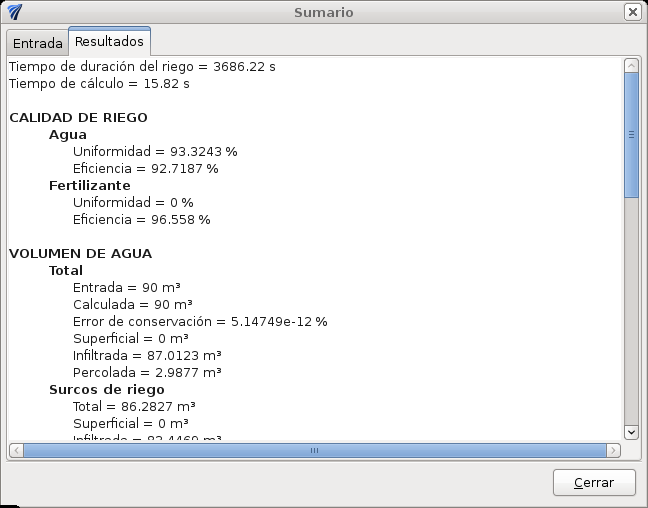
\includegraphics[width=0.45\textwidth]{images/sumario.png}
\qquad
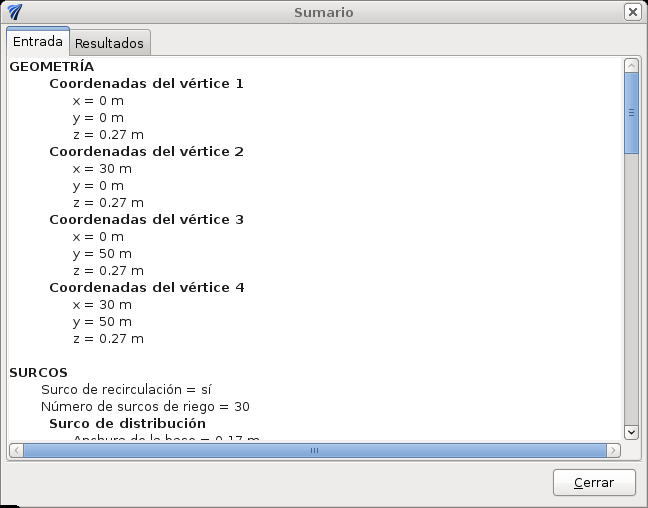
\includegraphics[width=0.45\textwidth]{images/sumario2.png}
\caption{Sumario de parámetros de entrada (Izquierda) y de resultados (Derecha)}\label{wInforme}
\end{center}
\end{figure}


%%%%%%%%%%%%%%%%%%%%%%%%%%%%%%%%%%%%%%%%%%%%%%%%%%%%%%%%%%%%%%%%%%%%%%%%%%%%%%%%%%%%%%%%%%%%%%%%%%%%%%%%5
